% !TEX program = xelatex

\documentclass[10pt, aspectratio=169]{beamer}

\usetheme[progressbar=none, numbering=none]{metropolis}
\usepackage{xcolor}
\usepackage{tikz}
\usetikzlibrary{calc,positioning}

% Paleta visual: industrial, escura, com acentos de sinal.
\definecolor{BaseBg}{HTML}{0B1020}
\definecolor{TopBar}{HTML}{111827}
\definecolor{PanelBg}{HTML}{172033}
\definecolor{PanelEdge}{HTML}{233047}
\definecolor{GridLine}{HTML}{26344F}
\definecolor{TextPrimary}{HTML}{F8FAFC}
\definecolor{TextMuted}{HTML}{AAB6C8}
\definecolor{AccentCyan}{HTML}{16D5D2}
\definecolor{SignalGreen}{HTML}{7DDC8A}
\definecolor{SignalAmber}{HTML}{F7B955}

\setbeamercolor{background canvas}{bg=BaseBg}
\setbeamercolor{normal text}{fg=TextPrimary,bg=BaseBg}
\setbeamercolor{frametitle}{fg=TextPrimary,bg=TopBar}
\setbeamercolor{title}{fg=TextPrimary}
\setbeamercolor{subtitle}{fg=TextMuted}
\setbeamercolor{author}{fg=TextMuted}
\setbeamercolor{institute}{fg=TextMuted}
\setbeamercolor{date}{fg=SignalAmber}
\setbeamercolor{alerted text}{fg=AccentCyan}
\setbeamercolor{block title}{fg=TextPrimary,bg=PanelEdge}
\setbeamercolor{block body}{fg=TextPrimary,bg=PanelBg}
\setbeamercolor{footline}{fg=TextMuted,bg=BaseBg}

\setbeamerfont{title}{size=\LARGE,series=\bfseries}
\setbeamerfont{subtitle}{size=\large}
\setbeamerfont{frametitle}{size=\large,series=\bfseries}
\setbeamerfont{block title}{series=\bfseries}
\setbeamerfont{footline}{size=\scriptsize}

\setbeamertemplate{navigation symbols}{}
\setbeamertemplate{blocks}[rounded][shadow=false]
\setbeamertemplate{itemize item}{\tikz\fill[AccentCyan] (0,0) circle (1.9pt);}
\setbeamertemplate{itemize subitem}{\tikz\fill[SignalGreen] (0,0) rectangle (3pt,3pt);}

% Fundo tecnico discreto: grade fina e planos de profundidade.
\setbeamertemplate{background}{
    
\begin{tikzpicture}
        \useasboundingbox (0,0) rectangle (\paperwidth,\paperheight);
        \fill[BaseBg] (0,0) rectangle (\paperwidth,\paperheight);

        \foreach \x in {0,0.55,...,16.6} {
            \draw[GridLine, opacity=0.18, line width=0.2pt] (\x,0) -- (\x,\paperheight);
        }
        \foreach \y in {0,0.55,...,9.4} {
            \draw[GridLine, opacity=0.18, line width=0.2pt] (0,\y) -- (\paperwidth,\y);
        }

        \fill[PanelBg, opacity=0.34] (12.45,0) -- (\paperwidth,0) -- (\paperwidth,\paperheight) -- (14.35,\paperheight) -- cycle;
        \draw[AccentCyan, opacity=0.18, line width=0.8pt] (12.55,0) -- (14.45,\paperheight);
        \draw[SignalGreen, opacity=0.16, line width=0.8pt] (13.25,0) -- (15.15,\paperheight);
        \fill[AccentCyan, opacity=0.22] (0,0) rectangle (\paperwidth,0.055);
    \end{tikzpicture}
}

\setbeamertemplate{frametitle}{
    \nointerlineskip
    \begin{beamercolorbox}[wd=\paperwidth,ht=0.95cm,dp=0.28cm,leftskip=0.82cm,rightskip=0.75cm]{frametitle}
        \usebeamerfont{frametitle}\insertframetitle
    \end{beamercolorbox}
    \begin{tikzpicture}[remember picture,overlay]
        \fill[AccentCyan] (current page.north west) rectangle ([xshift=0.16cm,yshift=-1.23cm]current page.north west);
        \fill[SignalGreen] ([xshift=0.16cm]current page.north west) rectangle ([xshift=0.23cm,yshift=-1.23cm]current page.north west);
        \draw[AccentCyan, opacity=0.5, line width=0.4pt] ([yshift=-1.23cm]current page.north west) -- ([yshift=-1.23cm]current page.north east);
    \end{tikzpicture}
}

\setbeamertemplate{footline}{
    \ifnum\value{framenumber}=1
    \else
        \begin{beamercolorbox}[wd=\paperwidth,ht=0.32cm,dp=0.16cm,leftskip=0.85cm,rightskip=0.85cm]{footline}
            \insertshorttitle\hfill\insertframenumber/\inserttotalframenumber
        \end{beamercolorbox}
    \fi
}

\setbeamertemplate{title page}{
    \begin{tikzpicture}[remember picture,overlay]
        \fill[AccentCyan] (current page.north west) rectangle ([xshift=0.18cm]current page.south west);
        \fill[SignalGreen] ([xshift=0.18cm]current page.north west) rectangle ([xshift=0.25cm]current page.south west);
        \fill[SignalAmber] ([xshift=0.25cm]current page.north west) rectangle ([xshift=0.30cm]current page.south west);

        \draw[AccentCyan, opacity=0.32, line width=1.1pt] ([xshift=0.85cm,yshift=-1.02cm]current page.north west) -- ([xshift=4.8cm,yshift=-1.02cm]current page.north west);
        \draw[SignalGreen, opacity=0.30, line width=1.1pt] ([xshift=0.85cm,yshift=-1.22cm]current page.north west) -- ([xshift=3.4cm,yshift=-1.22cm]current page.north west);
        \draw[SignalAmber, opacity=0.28, line width=1.1pt] ([xshift=0.85cm,yshift=-1.42cm]current page.north west) -- ([xshift=2.3cm,yshift=-1.42cm]current page.north west);

        \node[anchor=south east, text=PanelEdge, opacity=0.42, font=\fontsize{46}{46}\selectfont\bfseries]
            at ([xshift=-0.55cm,yshift=0.58cm]current page.south east) {PROFINET};
        \draw[PanelEdge, opacity=0.42, line width=0.5pt]
            ([xshift=-5.9cm,yshift=1.03cm]current page.south east) rectangle
            ([xshift=-0.65cm,yshift=2.08cm]current page.south east);
    \end{tikzpicture}

    \vspace*{1.35cm}
    \begin{minipage}{0.78\paperwidth}
        {\usebeamerfont{title}\usebeamercolor[fg]{title}\inserttitle\par}
        \vspace{0.28cm}
        {\usebeamerfont{subtitle}\usebeamercolor[fg]{subtitle}\insertsubtitle\par}
        \vspace{0.72cm}
        {\usebeamerfont{author}\usebeamercolor[fg]{author}\insertauthor\par}
        \vspace{0.10cm}
        {\usebeamerfont{institute}\usebeamercolor[fg]{institute}\insertinstitute\par}
        \vspace{0.35cm}
        {\usebeamerfont{date}\usebeamercolor[fg]{date}\insertdate\par}
    \end{minipage}
}

\newcommand{\slidechip}[2]{%
    \tikz[baseline=(chip.base)]\node[
        fill=#1,
        text=BaseBg,
        rounded corners=1.5pt,
        inner xsep=5pt,
        inner ysep=2pt,
        font=\scriptsize\bfseries
    ] (chip) {#2};%
}

\newcommand{\routebox}[3]{%
    \begin{tikzpicture}
        \node[
            fill=#1,
            text=TextPrimary,
            rounded corners=2pt,
            minimum width=2.65cm,
            minimum height=0.82cm,
            align=center,
            font=\footnotesize\bfseries
        ] {#2\\[-1pt]{\scriptsize #3}};
    \end{tikzpicture}%
}

% Informacoes da apresentacao
\title[PROFINET]{Pr\'atica: PROFINET e An\'alise de Tr\'afego}
\subtitle{Introdu\c{c}\~ao \`as Redes de Comunica\c{c}\~ao}
\author{Gabriel Silva}
\author{Victor Borga}
\institute{Universidade Federal de Pernambuco (UFPE)}
\date{Semestre 2026.1}

\begin{document}

\begin{frame}
    \titlepage
\end{frame}

\begin{frame}{Mapa da Aula}
    \small
    \slidechip{AccentCyan}{PROFINET}\hspace{0.18cm}
    \slidechip{SignalGreen}{Tempo Real}\hspace{0.18cm}
    \slidechip{SignalAmber}{Diagn\'ostico}

    \vspace{0.35cm}
    \begin{columns}[T,totalwidth=\textwidth]
        \begin{column}{0.46\textwidth}
            \begin{block}{Eixo te\'orico}
                \begin{itemize}
                    \item TI vs. TA e o problema do \alert{determinismo}.
                    \item Normas IEC 61158, IEC 61784-2 e IEC 62439-2.
                    \item PROFINET RT, IRT, NRT, PROFIsafe e DCP.
                \end{itemize}
            \end{block}
        \end{column}
        \begin{column}{0.46\textwidth}
            \begin{block}{Eixo pr\'atico}
                \begin{itemize}
                    \item Configura\c{c}\~ao no TIA Portal.
                    \item Acoplamento PLC-to-PLC com I-Device.
                    \item Captura de \texttt{pn\_rt}, \texttt{pn\_dcp} e TCP/IP no Wireshark.
                \end{itemize}
            \end{block}
        \end{column}
    \end{columns}
\end{frame}

\section[M\'odulo 1]{M\'odulo 1: Fundamentos das Redes Industriais}

\begin{frame}{M\'odulo 1: Fundamentos}
    \small
    \slidechip{AccentCyan}{Infraestrutura}\hspace{0.18cm}
    \slidechip{SignalGreen}{Determinismo}\hspace{0.18cm}
    \slidechip{SignalAmber}{Topologias}

    \vspace{0.35cm}
    \begin{block}{Objetivo do m\'odulo}
        Diferenciar redes de TI e TA, entender por que PROFINET n\~ao \'e apenas Ethernet comum e relacionar topologia f\'isica com disponibilidade da planta.
    \end{block}

    \begin{block}{Pergunta guia}
        O que muda quando a rede deixa de priorizar apenas entrega de dados e passa a exigir \alert{prazo de entrega}?
    \end{block}
\end{frame}

\begin{frame}{TI vs. TA: Requisitos Opostos}
    \small
    \begin{columns}[T,totalwidth=\textwidth]
        \begin{column}{0.46\textwidth}
            \begin{block}{Tecnologia da Informa\c{c}\~ao}
                \begin{itemize}
                    \item Baseada em Ethernet IEEE 802.3 e pilha TCP/IP.
                    \item Prioriza \textit{throughput}: volume total de dados por segundo.
                    \item TCP garante integridade com ACK, retransmiss\~ao e controle de fluxo.
                    \item Opera em modelo \textit{Best Effort}.
                \end{itemize}
            \end{block}
        \end{column}
        \begin{column}{0.46\textwidth}
            \begin{block}{Tecnologia da Automa\c{c}\~ao}
                \begin{itemize}
                    \item Controla CLPs, remotas de I/O, inversores e servos.
                    \item Prioriza tempo de ciclo previs\'ivel.
                    \item O dado correto atrasado pode ser tecnicamente inv\'alido.
                    \item Exige \alert{determinismo} e baixo jitter.
                \end{itemize}
            \end{block}
        \end{column}
    \end{columns}
\end{frame}

\begin{frame}{Best Effort e Determinismo}
    \small
    \begin{block}{Modelo \textit{Best Effort}}
        A rede tenta entregar o pacote \'integro, mas n\~ao oferece garantia matem\'atica sobre \textit{quando} ele chegar\'a. A lat\^encia varia e aparece como \textit{jitter}.
    \end{block}

    \begin{block}{Determinismo industrial}
        \'E a garantia de que um evento de comunica\c{c}\~ao ocorrer\'a dentro de um limite estrito: o tempo de ciclo de barramento \(t_{ciclo}\).
    \end{block}

    \begin{block}{Consequ\^encia de controle}
        Se um pacote chega depois do \textit{Watchdog Timer}, o receptor trata o dado como inv\'alido. O resultado pode ser alarme, trip, parada de emerg\^encia ou dano mec\^anico.
    \end{block}
\end{frame}

\begin{frame}{Paradigma PROFINET}
    \small
    \begin{block}{N\~ao \'e apenas um protocolo de software}
        PROFINET \'e uma arquitetura padronizada que combina requisitos de infraestrutura f\'isica, enlace Ethernet, aplica\c{c}\~ao industrial e perfis de tempo real.
    \end{block}

    \begin{columns}[T,totalwidth=\textwidth]
        \begin{column}{0.46\textwidth}
            \begin{block}{IEC 61158}
                \begin{itemize}
                    \item Define servi\c{c}os e protocolos de \textit{fieldbuses}.
                    \item Classifica PROFINET como Tipo 10.
                    \item Cobre camadas f\'isica, enlace e aplica\c{c}\~ao.
                \end{itemize}
            \end{block}
        \end{column}
        \begin{column}{0.46\textwidth}
            \begin{block}{IEC 61784-2}
                \begin{itemize}
                    \item Especifica perfis Ethernet de tempo real.
                    \item Exige suporte a VLAN e prioriza\c{c}\~ao.
                    \item Define crit\'erios de conformidade industrial.
                \end{itemize}
            \end{block}
        \end{column}
    \end{columns}
\end{frame}

\begin{frame}{Infraestrutura Industrial}
    \small
    \slidechip{AccentCyan}{IEC 61784-2}\hspace{0.18cm}
    \slidechip{SignalGreen}{EMI}\hspace{0.18cm}
    \slidechip{SignalAmber}{Switching}

    \vspace{0.35cm}
    \begin{block}{Meio f\'isico}
        Cabos blindados STP/SFTP Categoria 5e ou superior, condutores robustos para flex\~ao mec\^anica e conectores industriais RJ45 IP20 ou M12 codifica\c{c}\~ao D com prote\c{c}\~ao IP67.
    \end{block}

    \begin{block}{Comuta\c{c}\~ao}
        Switches industriais devem suportar \textit{Store-and-Forward} ou \textit{Cut-Through}, VLANs e prioriza\c{c}\~ao por \alert{IEEE 802.1Q}.
    \end{block}
\end{frame}

\begin{frame}{Canais L\'ogicos no Mesmo Cabo}
    \small
    \begin{columns}[T,totalwidth=\textwidth]
        \begin{column}{0.46\textwidth}
            \begin{block}{PROFINET NRT}
                \begin{itemize}
                    \item Canal aberto, n\~ao-tempo real.
                    \item Usa Ethernet II com EtherType \texttt{0x0800}.
                    \item Processa IP e TCP/UDP.
                    \item Usado para TIA Portal, diagn\'osticos e p\'aginas web.
                \end{itemize}
            \end{block}
        \end{column}
        \begin{column}{0.46\textwidth}
            \begin{block}{PROFINET RT}
                \begin{itemize}
                    \item Canal c\'iclico de tempo real.
                    \item Usa Ethernet II com \alert{EtherType \texttt{0x8892}}.
                    \item Ignora IP e TCP/UDP.
                    \item Reduz processamento interno a microsegundos.
                \end{itemize}
            \end{block}
        \end{column}
    \end{columns}
\end{frame}

\begin{frame}{Empacotamento: NRT vs. RT}
    \small
    \centering
    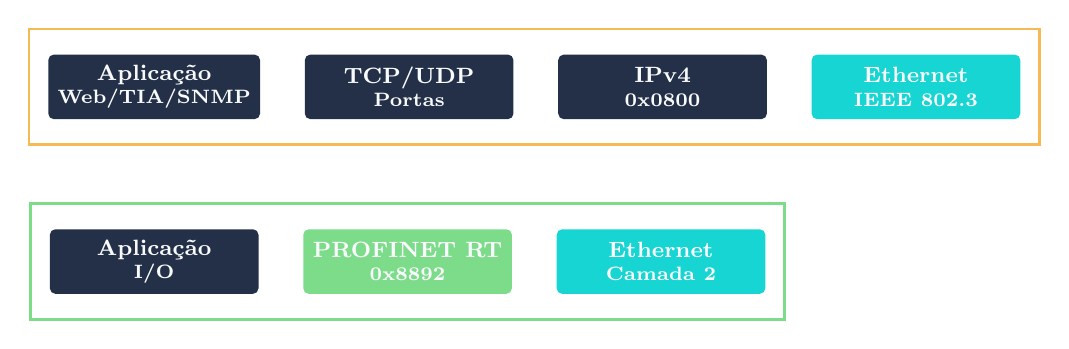
\begin{tikzpicture}[node distance=0.32cm]
        \node (n1) {\routebox{PanelEdge}{Aplica\c{c}\~ao}{Web/TIA/SNMP}};
        \node[right=0.32cm of n1] (n2) {\routebox{PanelEdge}{TCP/UDP}{Portas}};
        \node[right=0.32cm of n2] (n3) {\routebox{PanelEdge}{IPv4}{0x0800}};
        \node[right=0.32cm of n3] (n4) {\routebox{AccentCyan}{Ethernet}{IEEE 802.3}};

        \node[below=1.15cm of n1] (r1) {\routebox{PanelEdge}{Aplica\c{c}\~ao}{I/O}};
        \node[right=0.32cm of r1] (r2) {\routebox{SignalGreen}{PROFINET RT}{0x8892}};
        \node[right=0.32cm of r2] (r3) {\routebox{AccentCyan}{Ethernet}{Camada 2}};

        \draw[SignalAmber, line width=1pt] ($(n1.north west)+(-0.12,0.20)$) rectangle ($(n4.south east)+(0.12,-0.20)$);
        \draw[SignalGreen, line width=1pt] ($(r1.north west)+(-0.12,0.20)$) rectangle ($(r3.south east)+(0.12,-0.20)$);
    \end{tikzpicture}

    \vspace{0.35cm}
    \begin{block}{Leitura}
        O cabo \'e o mesmo, mas a pilha de processamento n\~ao \'e. O RT desvia as camadas 3 e 4 para preservar previsibilidade temporal.
    \end{block}
\end{frame}

\begin{frame}{Topologias Industriais}
    \small
    \begin{columns}[T,totalwidth=\textwidth]
        \begin{column}{0.46\textwidth}
            \begin{block}{Linha: \textit{Daisy Chain}}
                \begin{itemize}
                    \item Dispositivos com switches internos de 2 portas.
                    \item Reduz custo de cabeamento e dispensa switch central.
                    \item Falha em cabo ou n\'o intermedi\'ario isola dispositivos a jusante.
                \end{itemize}
            \end{block}
        \end{column}
        \begin{column}{0.46\textwidth}
            \begin{block}{Estrela}
                \begin{itemize}
                    \item Cada dispositivo vai a um switch industrial central.
                    \item Rompimento de um cabo afeta apenas um n\'o.
                    \item O switch central vira ponto \'unico de falha.
                \end{itemize}
            \end{block}
        \end{column}
    \end{columns}
\end{frame}

\begin{frame}{MRP: Anel com Alta Disponibilidade}
    \small
    \slidechip{AccentCyan}{IEC 62439-2}\hspace{0.18cm}
    \slidechip{SignalGreen}{MRM/MRC}\hspace{0.18cm}
    \slidechip{SignalAmber}{200 ms}

    \vspace{0.35cm}
    \begin{block}{Media Redundancy Protocol}
        O MRP une economia de cabeamento da linha com alta disponibilidade. A rede \'e fisicamente um anel, mas logicamente evita loop Ethernet.
    \end{block}

    \begin{columns}[T,totalwidth=\textwidth]
        \begin{column}{0.46\textwidth}
            \begin{block}{Pap\'eis}
                \begin{itemize}
                    \item MRM: \textit{Media Redundancy Manager}, geralmente o CLP mestre.
                    \item MRC: \textit{Media Redundancy Client}, todos os demais n\'os do anel.
                \end{itemize}
            \end{block}
        \end{column}
        \begin{column}{0.46\textwidth}
            \begin{block}{Opera\c{c}\~ao}
                \begin{itemize}
                    \item O MRM bloqueia logicamente uma porta.
                    \item Envia \textit{test frames} c\'iclicos.
                    \item Reconfigura a rota em at\'e \alert{200 ms} para 50 n\'os.
                \end{itemize}
            \end{block}
        \end{column}
    \end{columns}
\end{frame}

\begin{frame}{MRP: Falha e Reconfigura\c{c}\~ao}
    \small
    \begin{block}{Detec\c{c}\~ao}
        Quando um cabo rompe ou um MRC falha, os \textit{test frames} enviados pelo MRM deixam de retornar pela porta oposta.
    \end{block}

    \begin{block}{A\c{c}\~ao do Manager}
        O MRM desbloqueia a porta anteriormente inativa, restaurando conectividade pelo caminho alternativo.
    \end{block}

    \begin{block}{Reaprendizado}
        O MRM notifica os MRCs para limpar tabelas MAC/CAM, for\c{c}ando a rede a reaprender as novas rotas f\'isicas.
    \end{block}
\end{frame}

\section[M\'odulo 2]{M\'odulo 2: O Tr\'afego de Automa\c{c}\~ao}

\begin{frame}{M\'odulo 2: A Via R\'apida}
    \small
    \slidechip{AccentCyan}{PROFINET RT/IRT}\hspace{0.18cm}
    \slidechip{SignalGreen}{Camada 2}\hspace{0.18cm}
    \slidechip{SignalAmber}{QoS}

    \vspace{0.35cm}
    \begin{block}{Objetivo do m\'odulo}
        Entender como PROFINET reduz lat\^encia por \textit{bypass} de pilha, como prioriza tr\'afego em hardware e como os frames carregam dados de I/O c\'iclicos.
    \end{block}
\end{frame}

\begin{frame}{Bypass ao Modelo OSI}
    \small
    \begin{block}{Pilha reduzida}
        O PROFINET RT injeta dados da aplica\c{c}\~ao industrial diretamente na Camada 2. As camadas IP e TCP/UDP n\~ao participam do caminho de dados c\'iclico.
    \end{block}

    \begin{columns}[T,totalwidth=\textwidth]
        \begin{column}{0.46\textwidth}
            \begin{block}{Ganho}
                \begin{itemize}
                    \item Menor overhead de cabe\c{c}alho.
                    \item Menos ciclos de CPU do CLP.
                    \item Menos jitter introduzido por software.
                \end{itemize}
            \end{block}
        \end{column}
        \begin{column}{0.46\textwidth}
            \begin{block}{Endere\c{c}amento}
                \begin{itemize}
                    \item Sem IP no frame de tempo real.
                    \item Sem portas TCP/UDP.
                    \item Origem e destino pelo \alert{MAC Address}.
                \end{itemize}
            \end{block}
        \end{column}
    \end{columns}
\end{frame}

\begin{frame}{EtherType \texttt{0x8892}}
    \small
    \begin{block}{Campo de 2 bytes}
        No frame Ethernet II, o EtherType indica o protocolo encapsulado no payload. Para PROFINET RT, o valor obrigat\'orio \'e \alert{\texttt{0x8892}}.
    \end{block}

    \begin{block}{Filtro por hardware}
        Ao detectar \texttt{0x8892}, a NIC ou ASIC industrial direciona o pacote para buffers de I/O, sem acionar a pilha TCP/IP padr\~ao do sistema operacional do CLP.
    \end{block}

    \begin{block}{Resultado}
        O tr\'afego n\~ao disputa as mesmas rotinas de software usadas por web server, diagn\'ostico, sockets ou engenharia.
    \end{block}
\end{frame}

\begin{frame}{QoS via IEEE 802.1Q}
    \small
    \begin{block}{VLAN Tagging}
        PROFINET RT usa a extens\~ao IEEE 802.1Q. A tag adiciona 4 bytes ao frame e inclui o campo PCP, com 3 bits para prioridade.
    \end{block}

    \begin{columns}[T,totalwidth=\textwidth]
        \begin{column}{0.46\textwidth}
            \begin{block}{Priority Code Point}
                \begin{itemize}
                    \item 3 bits permitem 8 n\'iveis: 0 a 7.
                    \item Tr\'afego comum usa 0, \textit{Best Effort}.
                    \item PROFINET RT usa \alert{prioridade 6}.
                \end{itemize}
            \end{block}
        \end{column}
        \begin{column}{0.46\textwidth}
            \begin{block}{No switch}
                \begin{itemize}
                    \item PCP 6 vai para fila de alta prioridade.
                    \item O frame RT ultrapassa pacotes comuns.
                    \item Preserva o ciclo de controle sob carga.
                \end{itemize}
            \end{block}
        \end{column}
    \end{columns}
\end{frame}

\begin{frame}{Update Time e Watchdog}
    \small
    \begin{block}{Update Time}
        Intervalo em que o transmissor deve enviar um novo frame de dados. Valores comuns: 1 ms, 2 ms, 4 ms at\'e 512 ms.
    \end{block}

    \begin{block}{Watchdog Factor}
        Multiplicador inteiro que define quantos ciclos perdidos s\~ao tolerados. Valor padr\~ao comum: 3.
    \end{block}

    \begin{block}{Equa\c{c}\~ao operacional}
        \[
            \text{Watchdog Time} = \text{Update Time} \times \text{Watchdog Factor}
        \]
    \end{block}
\end{frame}

\begin{frame}{Falha de Watchdog}
    \small
    \begin{block}{Condi\c{c}\~ao de falha}
        Se o receptor atinge o \textit{Watchdog Time} sem receber o frame correto, assume perda de conex\~ao ou falha de provedor.
    \end{block}

    \begin{block}{Rea\c{c}\~ao no ecossistema Siemens}
        O CLP gera alarme de sistema, pode chamar OB86 e for\c{c}a m\'odulos de sa\'ida para o estado seguro configurado.
    \end{block}

    \begin{block}{Mensagem de engenharia}
        Em TA, a validade do dado depende de conte\'udo e tempo. Dado certo fora do prazo \'e dado errado.
    \end{block}
\end{frame}

\begin{frame}{DCP: Descoberta e Inicializa\c{c}\~ao}
    \small
    \slidechip{AccentCyan}{DCP}\hspace{0.18cm}
    \slidechip{SignalGreen}{Multicast}\hspace{0.18cm}
    \slidechip{SignalAmber}{Device Name}

    \vspace{0.35cm}
    \begin{block}{Discovery and Basic Configuration Protocol}
        O DCP parametriza dispositivos na Camada 2 antes da disponibilidade plena do canal TCP/IP. Ele associa \alert{PROFINET Device Name} ao MAC Address f\'isico.
    \end{block}

    \begin{block}{Nome de dispositivo}
        Dispositivos saem de f\'abrica sem IP definitivo. O identificador de planta \'e uma string como \texttt{et200sp-painel01}.
    \end{block}
\end{frame}

\begin{frame}{Sequ\^encia DCP}
    \small
    \begin{block}{Endere\c{c}o multicast}
        Frames DCP usam o destino PI \texttt{01:0E:CF:00:00:00}.
    \end{block}

    \begin{columns}[T,totalwidth=\textwidth]
        \begin{column}{0.30\textwidth}
            \begin{block}{1. Identify}
                O IO-Controller procura o \textit{Device Name} configurado no projeto.
            \end{block}
        \end{column}
        \begin{column}{0.30\textwidth}
            \begin{block}{2. Response}
                O dispositivo com nome correspondente responde ao MAC do CLP.
            \end{block}
        \end{column}
        \begin{column}{0.30\textwidth}
            \begin{block}{3. Set}
                O CLP grava IP, m\'ascara e gateway com base no nome validado.
            \end{block}
        \end{column}
    \end{columns}
\end{frame}

\begin{frame}{GSDML: Interoperabilidade}
    \small
    \begin{block}{General Station Description Markup Language}
        Arquivo XML usado para descrever matematicamente as propriedades, limites e diagn\'osticos de um dispositivo PROFINET.
    \end{block}

    \begin{columns}[T,totalwidth=\textwidth]
        \begin{column}{0.46\textwidth}
            \begin{block}{Identidade e estrutura}
                \begin{itemize}
                    \item \textit{Vendor ID} e \textit{Device ID}.
                    \item Slots e subslots suportados.
                    \item Tamanho de inputs e outputs em bytes.
                \end{itemize}
            \end{block}
        \end{column}
        \begin{column}{0.46\textwidth}
            \begin{block}{Engenharia e diagn\'ostico}
                \begin{itemize}
                    \item Faixas de opera\c{c}\~ao e filtros.
                    \item Par\^ametros de canais anal\'ogicos.
                    \item C\'odigos hexadecimais de falha f\'isica.
                \end{itemize}
            \end{block}
        \end{column}
    \end{columns}
\end{frame}

\begin{frame}{Anatomia PROFINET RT (1/2)}
    \small
    \begin{block}{Campos Ethernet}
        \begin{itemize}
            \item Preamble + SFD: 8 bytes de sincroniza\c{c}\~ao f\'isica.
            \item Destination MAC: 6 bytes.
            \item Source MAC: 6 bytes.
            \item VLAN IEEE 802.1Q: 4 bytes, com TPID \texttt{0x8100} e PCP 6.
            \item EtherType: 2 bytes, fixo em \alert{\texttt{0x8892}}.
        \end{itemize}
    \end{block}

    \begin{block}{Frame ID}
        Campo de 2 bytes. Valores de \texttt{0x8000} a \texttt{0xBBFF} indicam frames RT c\'iclicos de Classe 1, equivalentes ao contexto \texttt{RT\_CLASS\_1}.
    \end{block}
\end{frame}

\begin{frame}{Anatomia PROFINET RT (2/2)}
    \small
    \begin{block}{Payload e APDU Status}
        \begin{itemize}
            \item IO Data: 1 a 1440 bytes de vari\'aveis de processo.
            \item Cycle Counter: 2 bytes incrementais para detectar perda.
            \item Data Status: 1 byte com estado de RUN/STOP e validade.
            \item Transfer Status: 1 byte, usualmente \texttt{0x00}.
            \item FCS: 4 bytes CRC-32 no fechamento do frame.
        \end{itemize}
    \end{block}

    \begin{block}{Overhead}
        Em compara\c{c}\~ao com TCP/IP, o RT remove IP e TCP/UDP. O overhead estrutural de rede fica pr\'oximo de 26 bytes, antes do payload de I/O e do FCS.
    \end{block}
\end{frame}

\begin{frame}{PROFIsafe e Black Channel}
    \small
    \slidechip{AccentCyan}{IEC 61784-3-3}\hspace{0.18cm}
    \slidechip{SignalGreen}{Safety}\hspace{0.18cm}
    \slidechip{SignalAmber}{Black Channel}

    \vspace{0.35cm}
    \begin{block}{Princ\'ipio}
        PROFIsafe transmite dados de seguran\c{c}a funcional sobre a mesma infraestrutura PROFINET RT. A rede comum atua como \alert{Black Channel}: transporta bytes sem ser confi\'avel do ponto de vista de safety.
    \end{block}

    \begin{block}{Exemplos}
        Bot\~oes de emerg\^encia, cortinas de luz, chaves de porta, travas de seguran\c{c}a e sinais de parada segura.
    \end{block}
\end{frame}

\begin{frame}{Safety Trailer}
    \small
    \begin{block}{Controle dentro do payload}
        PROFIsafe consome 4 a 6 bytes do payload PROFINET para detectar repeti\c{c}\~ao, perda, atraso, corrup\c{c}\~ao ou inser\c{c}\~ao incorreta de pacotes.
    \end{block}

    \begin{columns}[T,totalwidth=\textwidth]
        \begin{column}{0.46\textwidth}
            \begin{block}{Temporiza\c{c}\~ao e sequ\^encia}
                \begin{itemize}
                    \item \textit{Consecutive Number} detecta ordem e duplicidade.
                    \item \texttt{F-WDTime} \'e watchdog dedicado de safety.
                \end{itemize}
            \end{block}
        \end{column}
        \begin{column}{0.46\textwidth}
            \begin{block}{Endere\c{c}amento e integridade}
                \begin{itemize}
                    \item F-Source-Address e F-Dest-Address validam pares l\'ogicos.
                    \item CRC de safety valida o conte\'udo cr\'itico.
                \end{itemize}
            \end{block}
        \end{column}
    \end{columns}
\end{frame}

\section[M\'odulo 3]{M\'odulo 3: O Tr\'afego de TI na Ind\'ustria}

\begin{frame}{M\'odulo 3: A Via Comum}
    \small
    \slidechip{AccentCyan}{NRT}\hspace{0.18cm}
    \slidechip{SignalGreen}{TCP/IP}\hspace{0.18cm}
    \slidechip{SignalAmber}{OUC}

    \vspace{0.35cm}
    \begin{block}{Objetivo do m\'odulo}
        Entender como tr\'afego TCP/IP convencional convive com PROFINET RT na mesma rede f\'isica, incluindo Modbus TCP, web server, SNMP e comunica\c{c}\~ao por sockets.
    \end{block}
\end{frame}

\begin{frame}{Canal TCP/IP Padr\~ao: NRT}
    \small
    \begin{block}{Identifica\c{c}\~ao}
        Frames NRT usam EtherType \texttt{0x0800}, que indica IPv4. O pacote segue para a pilha TCP/IP de software do CLP.
    \end{block}

    \begin{block}{Processamento}
        Ao contr\'ario de \texttt{0x8892}, o \texttt{0x0800} passa por rede e transporte: IP, TCP ou UDP, portas l\'ogicas, buffers e interrup\c{c}\~oes de firmware.
    \end{block}

    \begin{block}{Uso}
        Engenharia, diagn\'ostico, servidores web, SNMP, Modbus TCP, S7comm, sockets OUC e integra\c{c}\~oes com sistemas de TI.
    \end{block}
\end{frame}

\begin{frame}{Prioridade e Banda Residual}
    \small
    \begin{columns}[T,totalwidth=\textwidth]
        \begin{column}{0.46\textwidth}
            \begin{block}{Prioridade NRT}
                \begin{itemize}
                    \item PCP \texttt{0}: \textit{Best Effort}.
                    \item PCP \texttt{1}: \textit{Background}.
                    \item Menor prioridade que PROFINET RT com PCP 6.
                \end{itemize}
            \end{block}
        \end{column}
        \begin{column}{0.46\textwidth}
            \begin{block}{Aloca\c{c}\~ao}
                \begin{itemize}
                    \item Switches seguram NRT em buffers sob carga.
                    \item RT ocupa a janela temporal priorit\'aria.
                    \item IEC 61784-2 reserva banda para evitar \textit{starvation}.
                \end{itemize}
            \end{block}
        \end{column}
    \end{columns}
\end{frame}

\begin{frame}{Protocolos H\'ospedes}
    \small
    \begin{block}{Ideia central}
        Como PROFINET usa Ethernet padr\~ao na base, protocolos de aplica\c{c}\~ao sobre TCP/IP podem trafegar em paralelo no canal NRT.
    \end{block}

    \begin{columns}[T,totalwidth=\textwidth]
        \begin{column}{0.46\textwidth}
            \begin{block}{Modbus TCP}
                \begin{itemize}
                    \item IEC 61158 Type 8.
                    \item Camada 7 sobre TCP.
                    \item Porta l\'ogica \alert{502}.
                \end{itemize}
            \end{block}
        \end{column}
        \begin{column}{0.46\textwidth}
            \begin{block}{HTTP/HTTPS}
                \begin{itemize}
                    \item Porta TCP 80 para HTTP.
                    \item Porta TCP 443 para HTTPS/TLS.
                    \item Diagn\'ostico, firmware e p\'aginas de usu\'ario.
                \end{itemize}
            \end{block}
        \end{column}
    \end{columns}
\end{frame}

\begin{frame}{Encapsulamento Modbus TCP}
    \small
    \centering
    \resizebox{0.96\textwidth}{!}{%
    
\begin{tikzpicture}[node distance=0.28cm]
        \node (m1) {\routebox{AccentCyan}{Ethernet}{0x0800}};
        \node[right=0.26cm of m1] (m2) {\routebox{PanelEdge}{IP}{IPv4}};
        \node[right=0.26cm of m2] (m3) {\routebox{PanelEdge}{TCP}{Porta 502}};
        \node[right=0.26cm of m3] (m4) {\routebox{SignalGreen}{MBAP}{Header}};
        \node[right=0.26cm of m4] (m5) {\routebox{SignalAmber}{Modbus}{PDU}};
    \end{tikzpicture}
    }

    \vspace{0.4cm}
    \begin{block}{Transpar\^encia}
        O hardware PROFINET n\~ao altera o frame Modbus TCP. O CLP pode ser n\'o PROFINET via ASIC e cliente/servidor Modbus TCP via software.
    \end{block}
\end{frame}

\begin{frame}{SNMP e Gerenciamento}
    \small
    \begin{block}{SNMP}
        O Simple Network Management Protocol, RFC 1157, usa UDP nas portas 161 e 162 para consulta e notifica\c{c}\~ao.
    \end{block}

    \begin{block}{Uso industrial}
        Sistemas NMS interrogam objetos MIB em switches e CLPs para coletar estat\'isticas de porta, erros, carga de tr\'afego e condi\c{c}\~ao de links.
    \end{block}

    \begin{block}{Valor de diagn\'ostico}
        SNMP ajuda a separar falha de aplica\c{c}\~ao de falha f\'isica: atenua\c{c}\~ao, erro CRC, porta flapping e satura\c{c}\~ao.
    \end{block}
\end{frame}

\begin{frame}{Open User Communication}
    \small
    \slidechip{AccentCyan}{OUC}\hspace{0.18cm}
    \slidechip{SignalGreen}{Sockets}\hspace{0.18cm}
    \slidechip{SignalAmber}{TSEND/TRCV}

    \vspace{0.35cm}
    \begin{block}{Defini\c{c}\~ao}
        OUC \'e o conjunto de instru\c{c}\~oes nativas do CLP para abrir sockets TCP/UDP e trocar dados customizados sem depender de protocolos propriet\'arios.
    \end{block}

    \begin{block}{Estrutura de conex\~ao}
        Em Siemens, estruturas como \texttt{TCON\_IP\_v4} definem IP local/remoto, porta local/remota e protocolo de transporte.
    \end{block}
\end{frame}

\begin{frame}{OUC: TCP vs. UDP}
    \small
    \begin{columns}[T,totalwidth=\textwidth]
        \begin{column}{0.46\textwidth}
            \begin{block}{TCP - RFC 793}
                \begin{itemize}
                    \item Orientado \`a conex\~ao.
                    \item Usa \textit{three-way handshake}: SYN, SYN-ACK, ACK.
                    \item Garante ordem, retransmiss\~ao e controle de congestionamento.
                    \item Modelo \textit{stream-oriented}.
                \end{itemize}
            \end{block}
        \end{column}
        \begin{column}{0.46\textwidth}
            \begin{block}{UDP - RFC 768}
                \begin{itemize}
                    \item N\~ao orientado \`a conex\~ao.
                    \item Envia datagramas independentes.
                    \item Sem ACK, ordena\c{c}\~ao ou retransmiss\~ao.
                    \item Menor overhead e menor processamento.
                \end{itemize}
            \end{block}
        \end{column}
    \end{columns}
\end{frame}

\begin{frame}{Blocos OUC}
    \small
    \begin{columns}[T,totalwidth=\textwidth]
        \begin{column}{0.46\textwidth}
            \begin{block}{Conex\~ao}
                \begin{itemize}
                    \item \texttt{TCON}: abre socket; cliente ativo ou servidor passivo.
                    \item \texttt{TDISCON}: fecha conex\~ao e libera recursos.
                    \item Porta livre comum: 1025 a 65535.
                \end{itemize}
            \end{block}
        \end{column}
        \begin{column}{0.46\textwidth}
            \begin{block}{Dados}
                \begin{itemize}
                    \item \texttt{TSEND}/\texttt{TSEND\_C}: envia DB ou matriz de bytes.
                    \item \texttt{TRCV}/\texttt{TRCV\_C}: recebe dados em buffer.
                    \item Sufixo \texttt{\_C}: gest\~ao compacta de conex\~ao.
                \end{itemize}
            \end{block}
        \end{column}
    \end{columns}
\end{frame}

\section[M\'odulo 4]{M\'odulo 4: Ecossistema Siemens e Acoplamento de CLPs}

\begin{frame}{M\'odulo 4: Siemens e PLC-to-PLC}
    \small
    \slidechip{AccentCyan}{S7comm}\hspace{0.18cm}
    \slidechip{SignalGreen}{I-Device}\hspace{0.18cm}
    \slidechip{SignalAmber}{Segrega\c{c}\~ao}

    \vspace{0.35cm}
    \begin{block}{Objetivo do m\'odulo}
        Comparar mecanismos Siemens de comunica\c{c}\~ao propriet\'aria, transporte ISO on TCP, PUT/GET, acoplamento determin\'istico via I-Device e isolamento por m\'odulos CP.
    \end{block}
\end{frame}

\begin{frame}{S7comm vs. S7comm+}
    \small
    \begin{columns}[T,totalwidth=\textwidth]
        \begin{column}{0.46\textwidth}
            \begin{block}{S7comm cl\'assico}
                \begin{itemize}
                    \item Usado em S7-300 e S7-400.
                    \item Origem em MPI/PROFIBUS e adapta\c{c}\~ao a Ethernet.
                    \item Dados em \textit{plaintext}.
                    \item Exposto a leitura passiva e \textit{replay attacks}.
                \end{itemize}
            \end{block}
        \end{column}
        \begin{column}{0.46\textwidth}
            \begin{block}{S7comm+}
                \begin{itemize}
                    \item Introduzido em S7-1200/S7-1500.
                    \item Prote\c{c}\~ao em camada de aplica\c{c}\~ao.
                    \item Sess\~ao com desafio-resposta.
                    \item Criptografia e hashing do payload.
                \end{itemize}
            \end{block}
        \end{column}
    \end{columns}
\end{frame}

\begin{frame}{ISO on TCP: RFC 1006}
    \small
    \begin{block}{Problema}
        TCP \'e orientado a fluxo de bytes, sem delimitadores naturais de mensagem. Automa\c{c}\~ao baseada em PDUs precisa saber onde cada instru\c{c}\~ao come\c{c}a e termina.
    \end{block}

    \begin{block}{Solu\c{c}\~ao}
        A RFC 1006 adiciona TPKT e COTP sobre TCP, simulando servi\c{c}os ISO orientados a conex\~ao para transportar S7comm.
    \end{block}

    \begin{block}{Porta}
        A pilha Siemens S7comm usa tipicamente \alert{TCP 102}.
    \end{block}
\end{frame}

\begin{frame}{TPKT e COTP}
    \small
    \begin{columns}[T,totalwidth=\textwidth]
        \begin{column}{0.46\textwidth}
            \begin{block}{TPKT - 4 bytes}
                \begin{itemize}
                    \item Byte 0: vers\~ao \texttt{0x03}.
                    \item Byte 1: reservado \texttt{0x00}.
                    \item Bytes 2 e 3: comprimento total do pacote.
                \end{itemize}
            \end{block}
        \end{column}
        \begin{column}{0.46\textwidth}
            \begin{block}{COTP - 3 a 7 bytes}
                \begin{itemize}
                    \item Identifica tipo de TPDU.
                    \item Negocia conex\~ao e tamanho de PDU.
                    \item Gerencia fragmenta\c{c}\~ao de blocos S7comm.
                \end{itemize}
            \end{block}
        \end{column}
    \end{columns}
\end{frame}

\begin{frame}{Encapsulamento S7comm}
    \small
    \centering
    \resizebox{0.96\textwidth}{!}{%
    
\begin{tikzpicture}[node distance=0.25cm]
        \node (s1) {\routebox{AccentCyan}{Ethernet}{0x0800}};
        \node[right=0.24cm of s1] (s2) {\routebox{PanelEdge}{IP}{IPv4}};
        \node[right=0.24cm of s2] (s3) {\routebox{PanelEdge}{TCP}{102}};
        \node[right=0.24cm of s3] (s4) {\routebox{SignalAmber}{TPKT}{4 bytes}};
        \node[right=0.24cm of s4] (s5) {\routebox{SignalGreen}{COTP}{TPDU}};
        \node[right=0.24cm of s5] (s6) {\routebox{PanelEdge}{S7comm}{PDU}};
    \end{tikzpicture}
    }

    \vspace{0.35cm}
    \begin{block}{Leitura}
        S7comm n\~ao \'e PROFINET RT. Ele usa TCP/IP e participa do tr\'afego NRT, mesmo rodando na mesma infraestrutura f\'isica.
    \end{block}
\end{frame}

\begin{frame}{PUT e GET: Comunica\c{c}\~ao Unilateral}
    \small
    \begin{block}{Mecanismo}
        PUT e GET usam servi\c{c}os S7comm para transferir dados entre controladores sem l\'ogica ativa no lado servidor.
    \end{block}

    \begin{columns}[T,totalwidth=\textwidth]
        \begin{column}{0.46\textwidth}
            \begin{block}{GET}
                O cliente envia requisi\c{c}\~ao de leitura indicando \'area remota, por exemplo \texttt{DB10.DBX0.0}, e comprimento em bytes.
            \end{block}
        \end{column}
        \begin{column}{0.46\textwidth}
            \begin{block}{PUT}
                O cliente envia dados locais e endere\c{c}o de destino, sobrescrevendo a mem\'oria remota no CLP servidor.
            \end{block}
        \end{column}
    \end{columns}
\end{frame}

\begin{frame}{PUT/GET: Risco Operacional}
    \small
    \begin{block}{Independ\^encia do software}
        O CLP servidor pode ter mem\'oria lida ou escrita diretamente pelo firmware da interface. O programa do usu\'ario n\~ao precisa conter bloco de recep\c{c}\~ao.
    \end{block}

    \begin{block}{Risco}
        Qualquer dispositivo autorizado na rede e capaz de enviar S7comm na TCP 102 pode tentar acessar vari\'aveis cr\'iticas, se o recurso estiver habilitado.
    \end{block}

    \begin{block}{Controle no TIA Portal}
        Em S7-1200/S7-1500, \'e necess\'ario habilitar explicitamente: \textit{Permit access with PUT/GET communication from remote partner}.
    \end{block}
\end{frame}

\begin{frame}{I-Device: PLC como Remota}
    \small
    \begin{block}{Conceito}
        O recurso I-Device transforma a CPU de um CLP em um IO-Device inteligente para outro CLP, eliminando blocos de comunica\c{c}\~ao do programa do usu\'ario.
    \end{block}

    \begin{columns}[T,totalwidth=\textwidth]
        \begin{column}{0.46\textwidth}
            \begin{block}{IO-Controller}
                CLP mestre que gerencia ciclo, endere\c{c}amento l\'ogico e imagem de processo da rede.
            \end{block}
        \end{column}
        \begin{column}{0.46\textwidth}
            \begin{block}{I-Device / IO-Device}
                CLP subordinado que aparece como m\'odulo de I/O padr\~ao na rede PROFINET.
            \end{block}
        \end{column}
    \end{columns}
\end{frame}

\begin{frame}{Transfer Areas}
    \small
    \begin{block}{Imagem de processo}
        A troca de dados ocorre por buffers mapeados diretamente em inputs e outputs virtuais, com tamanhos fixos definidos pelo engenheiro.
    \end{block}

    \centering
    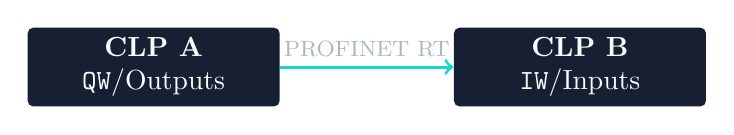
\begin{tikzpicture}
        \node[fill=PanelBg, rounded corners=2pt, minimum width=3.2cm, minimum height=1.0cm, align=center, text=TextPrimary] (q) {\textbf{CLP A}\\\texttt{QW}/Outputs};
        \node[fill=PanelBg, rounded corners=2pt, minimum width=3.2cm, minimum height=1.0cm, align=center, text=TextPrimary, right=2.2cm of q] (i) {\textbf{CLP B}\\\texttt{IW}/Inputs};
        \draw[->, AccentCyan, line width=1.1pt] (q) -- node[above, text=TextMuted, font=\footnotesize] {PROFINET RT} (i);
    \end{tikzpicture}

    \vspace{0.25cm}
    \begin{block}{Vantagem}
        Uma escrita em \texttt{QW} atravessa a rede e surge em \texttt{IW} no ciclo seguinte, com lat\^encia vinculada ao \textit{Update Time}.
    \end{block}
\end{frame}

\begin{frame}{I-Device vs. Blocos de Comunica\c{c}\~ao}
    \small
    \begin{columns}[T,totalwidth=\textwidth]
        \begin{column}{0.46\textwidth}
            \begin{block}{TSEND, TRCV, PUT}
                \begin{itemize}
                    \item Dependem de pilha TCP/IP ou S7comm.
                    \item Ass\'incronos em rela\c{c}\~ao ao ciclo de I/O.
                    \item Exigem l\'ogica de chamada, status e erro.
                \end{itemize}
            \end{block}
        \end{column}
        \begin{column}{0.46\textwidth}
            \begin{block}{I-Device}
                \begin{itemize}
                    \item Usa \alert{PROFINET RT \texttt{0x8892}}.
                    \item QoS prioridade 6.
                    \item Lat\^encia igual ao Update Time, podendo ser inferior a 2 ms.
                \end{itemize}
            \end{block}
        \end{column}
    \end{columns}
\end{frame}

\begin{frame}{Portas Integradas vs. M\'odulos CP}
    \small
    \begin{columns}[T,totalwidth=\textwidth]
        \begin{column}{0.46\textwidth}
            \begin{block}{Portas onboard}
                \begin{itemize}
                    \item Integradas \`a CPU.
                    \item Podem atuar como switch interno.
                    \item Tr\'afego externo pode consumir recursos da CPU.
                    \item DoS ou broadcast storm afetam o controle.
                \end{itemize}
            \end{block}
        \end{column}
        \begin{column}{0.46\textwidth}
            \begin{block}{CP / CM}
                \begin{itemize}
                    \item Processador e pilha de rede independentes.
                    \item Isolam TI e TA no hardware.
                    \item Passam vari\'aveis limpas pelo backplane.
                    \item Podem incluir firewall e filtros SPI.
                \end{itemize}
            \end{block}
        \end{column}
    \end{columns}
\end{frame}

\begin{frame}{Segrega\c{c}\~ao e Seguran\c{c}a}
    \small
    \begin{block}{Isolamento de redes}
        O tr\'afego da rede externa morre no m\'odulo CP. A CPU principal troca apenas dados controlados atrav\'es do barramento do rack.
    \end{block}

    \begin{block}{Firewall integrado}
        CPs industriais podem bloquear IPs, portas e padr\~oes de tr\'afego que n\~ao pertencem ao projeto de automa\c{c}\~ao.
    \end{block}

    \begin{block}{Prote\c{c}\~ao contra tempestades}
        Limitadores de broadcast e multicast impedem que falhas de TI contaminem o n\'ucleo de controle.
    \end{block}
\end{frame}

\section[M\'odulo 5]{M\'odulo 5: Diagn\'ostico e Ferramentas Pr\'aticas}

\begin{frame}{M\'odulo 5: Diagn\'ostico}
    \small
    \slidechip{AccentCyan}{Wireshark}\hspace{0.18cm}
    \slidechip{SignalGreen}{Port Mirroring}\hspace{0.18cm}
    \slidechip{SignalAmber}{Frames}

    \vspace{0.35cm}
    \begin{block}{Objetivo do m\'odulo}
        Usar captura de pacotes para diagnosticar falhas, intermit\^encias e gargalos em redes PROFINET, separando tr\'afego RT, NRT e DCP.
    \end{block}

    \begin{block}{Boa pr\'atica de captura}
        Preferir switch gerenci\'avel com \textit{Port Mirroring} ou SPAN. Capturar direto em linha sem TAP ou espelhamento pode alterar o comportamento da rede.
    \end{block}
\end{frame}

\begin{frame}{Wireshark: PROFINET RT}
    \small
    \begin{block}{Filtros}
        Use \texttt{pn\_rt} ou \texttt{eth.type == 0x8892}.
    \end{block}

    \begin{block}{Campos cr\'iticos}
        \begin{itemize}
            \item Frame ID: \texttt{0x8000} a \texttt{0xBBFF} confirma RT Classe 1.
            \item Cycle Counter: salto de numera\c{c}\~ao indica perda de pacote.
            \item Data Status: indica validade do dado e estado do provider.
        \end{itemize}
    \end{block}

    \begin{block}{Sintoma}
        Saltos como \texttt{4500} para \texttt{4502} sugerem \textit{packet drop}, ru\'ido EMI ou switch saturado.
    \end{block}
\end{frame}

\begin{frame}{Wireshark: PROFINET NRT}
    \small
    \begin{block}{Filtros}
        \texttt{ip.proto == 6} para TCP, \texttt{tcp.port == 102} para S7comm ou \texttt{tcp.port == 502} para Modbus TCP.
    \end{block}

    \begin{block}{Campos de diagn\'ostico}
        \begin{itemize}
            \item EtherType deve ser \texttt{0x0800}.
            \item Flags TCP \texttt{RST} ou retransmiss\~oes frequentes indicam queda l\'ogica, timeout ou instabilidade.
            \item TPKT deve iniciar com \texttt{0x03}; o campo Length deve bater com os bytes trafegados.
        \end{itemize}
    \end{block}
\end{frame}

\begin{frame}{Wireshark: PROFINET DCP}
    \small
    \begin{block}{Filtro}
        Use \texttt{pn\_dcp}.
    \end{block}

    \begin{block}{Campos cr\'iticos}
        \begin{itemize}
            \item MAC destino: \texttt{01:0E:CF:00:00:00}.
            \item Identify Request \texttt{0x05}: CLP procurando dispositivo.
            \item Identify Response \texttt{0x01}: dispositivo respondendo.
            \item Set Request \texttt{0x04}: grava\c{c}\~ao de IP baseada no nome.
        \end{itemize}
    \end{block}

    \begin{block}{Erro comum}
        Inspecione \texttt{Device Properties / Name of Station} para detectar diferen\c{c}a de grafia entre projeto TIA Portal e dispositivo real.
    \end{block}
\end{frame}

\begin{frame}{Checklist de Valida\c{c}\~ao em Laborat\'orio}
    \small
    \begin{columns}[T,totalwidth=\textwidth]
        \begin{column}{0.46\textwidth}
            \begin{block}{TIA Portal}
                \begin{itemize}
                    \item IPs na mesma \texttt{PN/IE\_1}.
                    \item I-Device associado ao IO-Controller.
                    \item \textit{Transfer areas} criadas.
                    \item Device Name gravado via DCP.
                \end{itemize}
            \end{block}
        \end{column}
        \begin{column}{0.46\textwidth}
            \begin{block}{Wireshark}
                \begin{itemize}
                    \item \texttt{pn\_dcp}: identifica\c{c}\~ao e atribui\c{c}\~ao de nome.
                    \item \texttt{pn\_rt}: fluxo c\'iclico sem IPv4.
                    \item \texttt{tcp.port == 102}: S7comm/NRT.
                    \item \texttt{tcp.port == 502}: Modbus TCP.
                \end{itemize}
            \end{block}
        \end{column}
    \end{columns}
\end{frame}

\begin{frame}{Fechamento}
    \small
    \begin{block}{S\'intese}
        PROFINET combina Ethernet industrial, prioriza\c{c}\~ao IEEE 802.1Q, frames de Camada 2, canal TCP/IP paralelo e perfis especializados como PROFIsafe.
    \end{block}

    \begin{block}{Ideia essencial}
        A diferen\c{c}a entre TI e TA n\~ao \'e apenas velocidade. \'E previsibilidade temporal, comportamento sob falha e controle do caminho de processamento.
    \end{block}

    \begin{block}{Prova pr\'atica}
        Quando o Wireshark mostra \texttt{EtherType 0x8892} sem IPv4, ele est\'a mostrando a decis\~ao arquitetural que permite o \alert{determinismo} do PROFINET RT.
    \end{block}
\end{frame}

\end{document}
